\documentclass[a4]{article}
\usepackage{gnuplottex}
\usepackage{csvsimple}
\usepackage{subcaption}
\usepackage{amsmath}
\usepackage{listings}
\usepackage{xcolor}

\title{COMP25212 System Architecture}
\author{}
\begin{document}
\maketitle

\subsection*{Q1.}
5.2\% of instructions accounted for 90\% of the executed instructions. Using a simple python script I summed the number of times each instruction was executed then sorted by most executed
and tallied number of executions until it exceeded 90\% of the total executions. I then dived the number of instructions I had tallied and divided by total instructions.\newline
answer:\textbf{5.2\%}

\subsection*{Q2.}
428065 branches where taken\newline
answer:\textbf{428065}

\subsection*{Q3.}
3423933 instructions where executed so on average 8.00 instructions are run before the pc is reloaded.\newline
answer:\textbf{8.00}

\subsection*{Q4.}
856130 (2 x 428065) instructions where wasted making the 20.0\% of instructions wasted.\newline
answer:\textbf{20.0\%}

\subsection*{Q5.}
answer:\textbf{89.3\%}

\subsection*{Q6.}
answer:\textbf{2.6\%}\newline
Of the branches taken only 45859 where not B branches so using the calculation Q4 we get a new percent of wasted time.\newline

\subsection*{Q7.}
Branches at the end of loops are imperfect because at the end of a loop the branch behave differently than previously expected and only does so once. Sometimes branches 
are effected by unpredictable external input and cant be predicted.

\subsection*{Q8.}
answer:\textbf{428065:239802}\newline

\subsection*{Q9.}
answer:\textbf{272241:239802}\newline

\subsection*{Q10.}
answer:\newline
\textbf{forward: 119969:154253}\newline
\textbf{backward: 146936:59812}\newline

\subsection*{Q11.}
When taking a backwards branch predict it is taken as the majority of the time it is, and when forwards assume it isnt taken. This is more effective on backwards branches.

\subsection*{Q12.}
A high degree of associativity is preferable as the cache is usualy very small and can still be fast and due to its size means direct mapped migh result in many collisions.

\subsection*{Q13.}
1 word or 32 bits as that is the size of the address expected by the branch.

\subsection*{Q14.}
I cache all invariant branches using a cyclic cache replacement policy. If cached then it is assumed that the branch is taken.
\begin{lstlisting}[language = python]
    cycle = 0
    cachesize = 15
    cache = []
    for i in range(cachesize):
        cache.append(None)
    
    def searchCache(key): 
        global cycle, cachesize, cache
        for entry in cache:
            if entry == key:
                return True
        return False
    
    def addCache(key):  #cycle cache replacement
        global cycle, cachesize, cache
        cache[cycle] = key
        cycle += 1
        if cycle == cachesize:
            cycle = 0
    
    f = open("block_profile", "r")
    lines = []
    noPenalty = 0 
    penalty = 0
    for line in f:
        lines.append(list(filter(lambda a:a != " " and a != "", line.split(" "))))
    for line in lines:
        if line[0] == "B":
            hit = searchCache(line[2])
            if hit:
                if line.count("not") == 0:
                    noPenalty += 1  #cache hit and taken
                else:
                    penalty += 1    #cache hit but not taken
            else:
                if line.count("not") > 0:
                    noPenalty += 1  #no cache hit not taken
                else:
                    penalty += 1 #no cache hit is taken
                    addCache(line[2]) #no hit and taken so store in cache
        else:
            if line.count("not") > 0:
                noPenalty += 1  # not invariant and not taken
            else:
                penalty += 1    #not invariant is taken
    print(penalty)
    print(noPenalty)
\end{lstlisting}

\subsection*{Q15.}
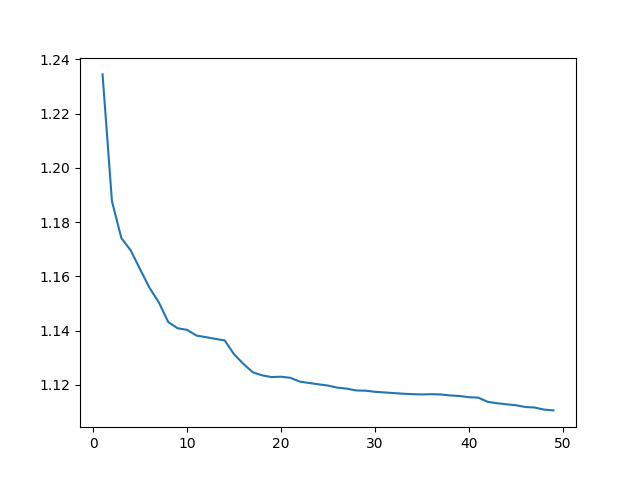
\includegraphics{phase2graph.png}

\subsection*{Q16.}
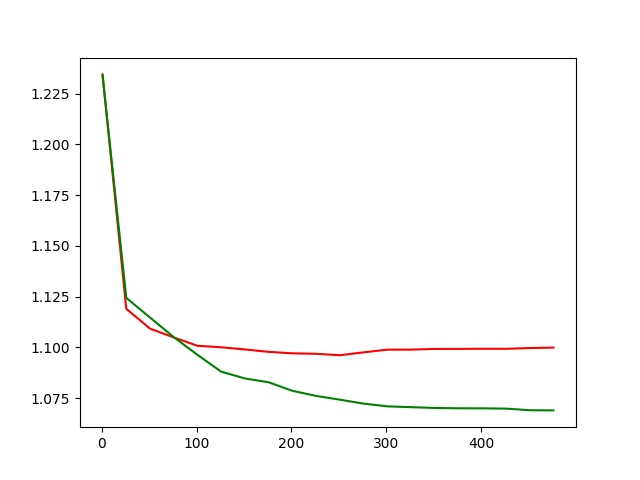
\includegraphics{phase3graph.png}
\color{green} -----\color{black} State aproach\newline
\color{red} -----\color{black} Non state aproach 

\subsection*{Q17.}
answer:\textbf{0.59049}\newline

\subsection*{Q18.}
One one simple predictor is a loop predictor. Most loops will itterate x many times then not once and in the case of loops x is known and each loop can correctly be 
predicted including the last branch unlike if you used a simple dynamic branch predictor.

\subsection*{Q19.}
Returns from functions use a return stack that predicts the function will return to the place it wascalled from. The return stack is a mirror of the call stack.
This means the prediction can handle recursion as simply the same return will be pushed to the stack mutiple times. Another option is a local branch predictor 
that uses a history buffer for each branch and will predict based on the history. This improves over the state approach as you have access to more data and can study patern.

\subsection*{Q20.}
A switch case statement or some if statements also qualify. 

%% Any raw data or code scripts you want to present should be included as appendices.
\end{document}
